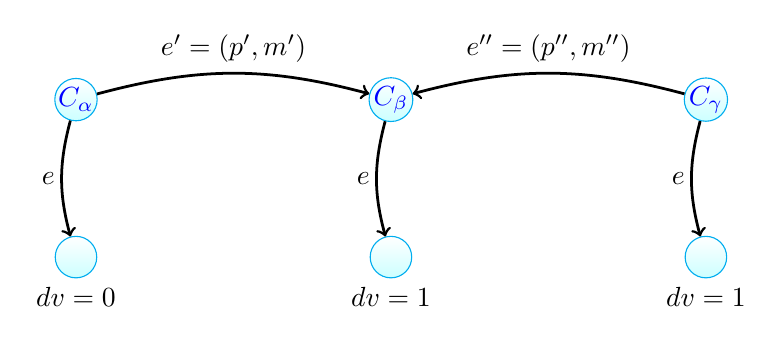
\begin{tikzpicture}


\tikzset{label/.style={minimum size=15pt,inner sep=0pt,},}
\tikzset{conf/.style={circle,minimum size=15pt,inner sep=0pt,draw, top color=white ,bottom color=cyan!20, cyan,text=blue},}

\tikzset{camminoUp/.style={->, line width=1pt, snake=coil, segment amplitude=1pt, segment aspect=0, segment length=4mm}}
\tikzset{camminoDown/.style={->, line width=1pt, snake=coil, mirror snake, segment amplitude=1pt, segment aspect=0, segment length=4mm}}
	\draw
		(0,0) node[conf] (c1) {$C_\alpha$}
		(4,0) node[conf] (c2) {$C_\beta$}
		(8,0) node[conf] (c3) {$C_\gamma$}
		
		(0,-2) node[conf] (d1) {} (0,-2.5)node[label]{$dv=0$}
		(4,-2) node[conf] (d2) {} (4,-2.5)node[label]{$dv=1$}
		(8,-2) node[conf] (d3) {} (8,-2.5)node[label]{$dv=1$}
		
;


\draw[->,line width=1pt](c1) to [bend left=15]  (c2);\draw(2,0.65)node[label]{$e'=(p',m')$};
\draw[->,line width=1pt](c3) to [bend right=15]  (c2);\draw(6,0.65)node[label]{$e''=(p'',m'')$};
\draw[->,line width=1pt](c1) to [bend right=15]  (d1);\draw(-0.35,-1)node[label]{$e$};
\draw[->,line width=1pt](c2) to [bend right=15]  (d2);\draw(3.65,-1)node[label]{$e$};
\draw[->,line width=1pt](c3) to [bend right=15]  (d3);\draw(7.65,-1)node[label]{$e$};





\end{tikzpicture}